\documentclass{beamer}
\beamertemplatenavigationsymbolsempty
\usecolortheme{beaver}
\setbeamertemplate{blocks}[rounded=true, shadow=true]
\setbeamertemplate{footline}[page number]
\usepackage[utf8]{inputenc}
\usepackage{amsmath,amssymb}
\usepackage{hyperref}
\usepackage{biblatex}
\addbibresource{sample.bib}

% Title Page Information
\title{Neural architecture search with target hardware control}
\author{Firsov Sergey \\ Supervisor: Oleg Bakhteev, PhD}
\institute{Moscow Institute of Physics and Technology}
\date{2024}

\begin{document}

\begin{frame}
    \titlepage
\end{frame}

%%%%%%%%%%%%%%%%%%%%%%%%%%%%%%%%%%%%%%%%%%%%%%%%%%%%
\begin{frame}{Problem}
\begin{itemize}
    \item \textbf{Neural Architecture Search:} 
    Automate the design of neural network architectures to solve ML tasks
    \item \textbf{Goal:} Identify architectures that optimize task performance while balancing computational cost and resource efficiency.
    \item \textbf{Challenges:}
    \begin{itemize}
        \item \textbf{Vast Search Space:} The number of possible architectures grows exponentially with model complexity.
        \item \textbf{Trade-offs:} Balancing accuracy, model complexity, and hardware efficiency.
        \item \textbf{Resource Constraints:} Models must perform well within predefined latency, memory, or energy limits.
        \item \textbf{Multiple result:} Getting architectures as a function of complexity, thereby having multiple architectures in one answer.
    \end{itemize}
    
\end{itemize}
\end{frame}


\begin{frame}{Existing Methods}
Exhaustive search for optimal architectures using: 
\begin{itemize}
        \item reinforcement learning
        \item evolutionary algorithms
        \item gradient-based methods
\end{itemize}

\textbf{Differentiable Architecture Search (DARTS):}
\begin{itemize}

        \item formulates NAS as a continuous optimization problem, enabling gradient-based search.
        \item reduces computational cost by relaxing the discrete search space into a differentiable one.

\end{itemize}

\textbf{Problems with Existing Methods:}
\begin{itemize}

        \item \textbf{accuracy vs. complexity:} often focus solely on accuracy, neglecting the importance of model complexity control.
        \item \textbf{hardware constraints ignored:} lack of mechanisms to account for real-world hardware constraints like latency or energy consumption.
        \item \textbf{limited flexibility:} insufficient control over the trade-off between accuracy and resource efficiency.

\end{itemize}
\end{frame}



%%%%%%%%%%%%%%%%%%%%%%%%%%%%%%%%%%%%%%%%%%%%%%%%%%%%

\begin{frame}{Architecture of solution}

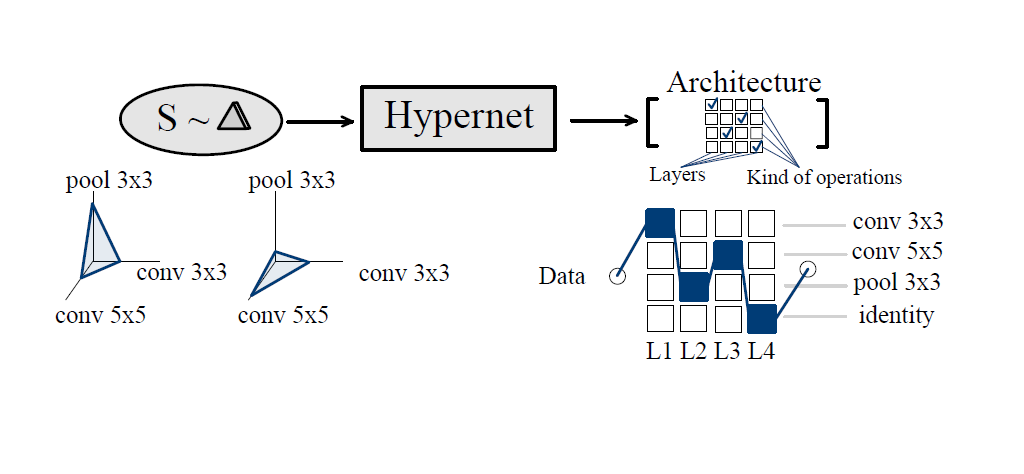
\includegraphics[width=1\linewidth]{picture.png}

\end{frame}

%%%%%%%%%%%%%%%%%%%%%%%%%%%%%%%%%%%%%%%%%%%%%%%%%%%%

\begin{frame}{Step 1: Complexity-Aware Architecture Representation}
\begin{itemize}
    \item Architectural parameters \(\boldsymbol{\alpha}\) - functions from complexity parameter \(\lambda\) to architectural space \(  \mathcal{A} \):
    \[
    \boldsymbol{\alpha}: \lambda \to \mathcal{A}.
    \]
    \item Generates multiple architectures with varying complexities in a single optimization process.
    \item Ensures flexibility in architecture design across resource constraints.
\end{itemize}
\end{frame}

%%%%%%%%%%%%%%%%%%%%%%%%%%%%%%%%%%%%%%%%%%%%%%%%%%%%

\begin{frame}{Step 2: Simplex-Based Complexity Control}
\begin{itemize}
    \item Replace scalar complexity parameter (\(\lambda\)) with a simplex representation:
    \[
    \boldsymbol{S} \in \Delta^{k-1}.
    \]
    This makes complexity management more flexible for different types of operations.  
    \item \(\Delta^{k-1}\): \((k-1)\)-dimensional simplex, where \(k\) is the number of operations: now we have a different regularization coefficient for each operation.
    \item Sampling via Gumbel-Softmax enables differentiable selection of operations:
    \[
    \boldsymbol{S} \sim \text{GumbelSoftmax}(\boldsymbol{\theta}).
    \]
\end{itemize}
\end{frame}

%%%%%%%%%%%%%%%%%%%%%%%%%%%%%%%%%%%%%%%%%%%%%%%%%%%%

\begin{frame}{Step 3: Hardware-Aware Latency Regularization}
\begin{itemize}
    \item \textbf{Latency-Aware Optimization:}  
    Introduce a term in the loss function to account for operation latency on target hardware.
    \[
    \text{Loss} = L + \kappa \cdot \text{Latency}(\boldsymbol{\alpha(S)}),
    \]
    where \(\kappa\) is a regularization coefficient.
    \item \textbf{Purpose:}  
    \begin{itemize}
        \item Ensure the resulting architecture meets real-world hardware constraints, such as inference time limits.
        \item Optimize architectures not just for accuracy, but for deployment feasibility on specific devices.
    \end{itemize}
\end{itemize}
\end{frame}


%%%%%%%%%%%%%%%%%%%%%%%%%%%%%%%%%%%%%%%%%%%%%%%%%%%%


\begin{frame}{Final Loss Function}
\begin{itemize}
    \item \textbf{Optimization problem:} minimize functional
\end{itemize}

    \[
    \mathbb{E}_{\boldsymbol{S} \sim \text{GumbelSoftmax}} \big[L(\boldsymbol{w}^*(\boldsymbol{S}), \boldsymbol{\alpha}(\boldsymbol{S})) + \lambda \cdot \text{Reg}(\boldsymbol{\alpha}(\boldsymbol{S}))) + \kappa \cdot \text{Latency}(\boldsymbol{\alpha}(\boldsymbol{S})))\big].
    \]
\begin{itemize}
    \item \textbf{Key Insights:}
    \begin{itemize}
        \item by using complexity dependence architecture parameters we generate multiple architectures in a single optimization process, 
        \item by replacing the scalar complexity parameter with the simplex representation, we achieve finer control over architectural complexity, enabling flexible optimization across a range of hardware and resource constraints,
        \item by using latency lookup table, we can control hardware constraints.
    \end{itemize}
\end{itemize}
\end{frame}

%%%%%%%%%%%%%%%%%%%%%%%%%%%%%%%%%%%%%%%%%%%%%%%%%%%%


\begin{frame}{Planned Experiments}
\begin{itemize}
    \item Validate the proposed method on:
    \begin{itemize}
        \item Image classification benchmarks (e.g.,fmnist, CIFAR-10).
        \item Hardware-specific performance metrics.
    \end{itemize}
    \item Compare against:
    \begin{itemize}
        \item Baseline methods (DARTS, ProxylessNAS, FBNet).
        \item Metrics: Accuracy, latency, and complexity.
    \end{itemize}
    \item Evaluate trade-offs between accuracy and latency.
\end{itemize}
\end{frame}

%%%%%%%%%%%%%%%%%%%%%%%%%%%%%%%%%%%%%%%%%%%%%%%%%%%%


\begin{frame}{Results}
\begin{itemize}
    \item Placeholder for experimental results.
    \item Future work: Analyze results and provide insights.
\end{itemize}
\end{frame}

\begin{frame}[allowframebreaks]{References}
    \printbibliography
\end{frame}

\end{document}
